\documentclass[12pt, A4]{article}
\usepackage[utf8]{inputenc}
\usepackage{geometry}
\geometry{
	a4paper,
	left=15mm,
	right=15mm,
	top=25mm,
	bottom=20mm
}
\usepackage{amsmath}
\usepackage{amsfonts}
\usepackage{amssymb}
\usepackage{graphicx}
\graphicspath{ {./images/} }
\usepackage{hyperref}
\hypersetup{
	colorlinks=true,
	linkcolor=black,
	filecolor=magenta,      
	urlcolor=cyan,
	pdfpagemode=FullScreen,
}

\makeatletter
\renewcommand{\theenumi}{\roman{enumi}}

\newcommand{\indep}{\perp \!\!\! \perp}

\newcommand{\sq}{$\square$}
\newcommand{\rmk}{$\surd$}
\newcommand{\trick}{$\bigstar$}
\newcommand{\N}{\mathbb{N}}
\newcommand{\Q}{\mathbb{Q}}
\newcommand{\R}{\mathbb{R}}
\newcommand{\U}{\mathcal{U}}
\newcommand{\V}{\mathcal{V}}
\newcommand{\A}{\mathcal{A}}
\newcommand{\B}{\mathcal{B}}
\newcommand{\C}{\mathcal{C}}
\newcommand{\F}{\mathcal{F}}
\newcommand{\LL}{\mathcal{L}}
\newcommand{\open}{\underset{open}{\subset}}
\newcommand{\closed}{\underset{closed}{\subset}}
\newcommand{\subsp}{\underset{subsp}{\subset}}
\newcommand{\seq}{\underset{seq}{\subset}}
\newcommand{\cl}{\overline}
\newcommand{\diff}{\,\backslash\,}
\newcommand{\union}{\,\cup\,}
\newcommand{\intersect}{\,\cap\,}
\newcommand{\exist}{\exists\,}
\newcommand{\convp}{\overset{P}{\rightarrow}}
\newcommand{\convd}{\overset{D}{\rightarrow}}
\newcommand{\foranyn}{\quad \forall \, n\in \N}


\begin{document}
\begin{titlepage}
	\begin{center}
		\vspace*{5cm}
		\textbf{\Large Probability theory \MakeUppercase{\romannumeral 2} Facts}
		\\
		\vspace{1.5cm}
		\textbf{Taeyoung Chang}
		\vfill
		Textbook : Rick Durrett $\ulcorner$ Probability : Theory and Examples $\lrcorner$ 5th edition
		\\
		\vspace{0.8cm}
		Last Update : \today
		\vspace*{3cm}
		\thispagestyle{empty}
	\end{center}
\end{titlepage}
\tableofcontents
\clearpage

\section{Conditional Expectation}
\smallskip
\begin{itemize}
    \item Projection Thm for Hilbert Space
    \begin{itemize}
        \item If $E$ is a Hilbert space and $M\subset E$ is closed and convex, then for any $y\in E$, \\$\exists$ a unique $w\in M$ s.t. $\|y-w\|=d(y, M):=\inf\{\|y-v\|:v\in M\}$. \\ Denote it as $w=proj_{M}y$ \; i.e. $w$ is a projection of $y$ onto $M$ . 
		\item If $E$ is a Hilbert space and $M\subset E$ is a closed vector subspace, then for any $y\in E$, 
		\begin{enumerate}
			\item $\exists$ a unique decomposition $y=w+v$ with $w=proj_M y\in M$ and $v\in M^{\perp}$ 
			\item For $w\in M$, \quad $ w=proj_M y \Leftrightarrow \langle y-w, z\rangle =0 \quad  \forall \, z\in M$
		\end{enumerate}
	\end{itemize}
	\item[*] $\LL^2:=\{$ Random Variable $ X : E(X^2)=\int X^2\,dP<\infty\}$
	\item[\rmk] If $X\in \LL^2$ then $E|X|<\infty$ \; i.e. every element of $\LL^2$ is integrable.
	\begin{itemize}
		\item[\trick] Trick : $|X|\leq X^2+\frac{1}{4}$
	\end{itemize} 
	\item[\rmk] $\LL^2$ is a vector space
	\begin{itemize}
		\item[\trick] Trick : inequality $(aX+bY)^2\leq 2(a^2 X^2+b^2Y^2)$
	\end{itemize}  
	\item $\LL^2$ is a Hilbert space with inner product $\langle X, Y\rangle = E(XY)$ 
	\begin{itemize}
		\item[\trick] Trick :  Cauchy seq. having a subseq. converging to a point converges to the point. 
	\end{itemize}
	\item Lemma for proving $\LL^2$ is a complete normed space.
	\begin{itemize}
		\item If $\{X_n\}\seq \LL^2$ and $\|X_n-X_{n+1}\|\leq 2^{-n}\foranyn$ then $\exist X\in \LL^2$ s.t. $X_n\rightarrow X \quad a.s.$ and $\|X_n-X\|\rightarrow 0$ \;i.e. $X_n\rightarrow X$ in $\LL^2$.
		\begin{itemize}
			\item[\trick] Lemma : If a random varaible $Z$ satisfies $Z\geq 0$ and $E(Z)<\infty$ then $Z<\infty \quad a.s.$ 
		\end{itemize}
	\end{itemize}
	\item[*] For $X\in \LL^2$, \; $\LL^2(X):=\{g(X)\,|\, g:\R\rightarrow \R$ is a Borel function, $E[(g(X))^2]<\infty\}$
	\item[\rmk] For $X\in \LL^2$, \; $\LL^2(X)$ is a vector subspace of $\LL^2$.
	\item For $X\in \LL^2$, \; $\LL^2(X)$ is a closed vector subspace of $\LL^2$ so that $\LL^2(X)$ is also a Hilbert space. 
	\item[*] Geometric definition for conditional expectation
	\begin{itemize}
		\item For $X , Y\in \LL^2$, define $E[Y|X]=Proj_{\LL^2(X)}Y$
		\item $E[Y|X]=g(X)\; a.s.$ for some Borel function $g$
		\item $\|Y-E[Y|X]\|=\min_{h(X)\in \LL^2(X)}\|Y-h(X)\|$ \\ i.e. $E[(Y-E[Y|X])^2]\leq E[(Y-h(X))^2]\quad \forall\; h(X)\in \LL^2$
		\item For $g(X)\in \LL^2(X)$, \quad $g(X)=E[Y|X]\Leftrightarrow \langle Y-g(X), h(X)\rangle=0 \quad \forall\; h(X)\in \LL^2 \\ \Leftrightarrow E[(Y-g(X))h(X)]=0 \quad \forall \;h(X)\in \LL^2$
	\end{itemize} 
	\item Elementary properties of conditional expectation from geometric definition
	\begin{itemize}
		\item If $X, Y, Z\in \LL^2$ then the followings are true.
		\begin{enumerate}
			\item $E[c|X]=c\; a.s. \quad \forall \; c\in \R$
			\item $E[\alpha Y+\beta Z |X]=\alpha E[Y|X]+\beta E[Z|X]\quad \forall \alpha, \beta\in \R$
			\item $E[Y|X]=E[Y]$ if $X$ and $Y$ are independent.
			\item $E[g(X)Y|X]=g(X)E[Y|X]$ if $g$ satisfies $g(X)\in \LL^2(X)$ and $\sup_x |g(x)|<\infty$
			\item $E[E[Y|X]]=E[Y]$
			\item[\rmk] In fact, the additional assumption about boundedness of $g$ in (\romannumeral 4) is not necessary. We will see later.
		\end{enumerate}
	\end{itemize}
	\item Extending the definition from $\LL^2$ to all integrable functions
	\begin{align*}
		E[\{Y-E[Y|X]\}I(X\in A)] &=0 \quad \forall \; A\in \B(\R) \quad \because I(X\in A)\in \LL^2(X) \\
		\int_{(X\in A)}Y\, dP &= \int_{(X\in A)}E[Y|X]\, dP \quad \forall \; A\in \B(\R) \\
		\int_B Y\, dP&=\int_B E[Y|X]\, dP \quad \forall \; B\in \sigma(X)
	\end{align*}
	\begin{itemize}
		\item $E[Y|X]\in \sigma(X)$ and $\int_B Y\, dP=\int_B E[Y|X]\, dP \quad \forall \; B\in \sigma(X)$. Such r.v. is unique in the sense that if any r.v. $Z$ satisfies $Z\in \sigma(X)$ and $\int_B Y\, dP=\int_B Z\, dP \quad \forall \; B\in \sigma(X)$ then $Z=E[Y|X]\; a.s.$ provided $E|Y|<\infty$
		\item From the theory on $\LL^2$ space, we get geometric understanding about conditional expectation. But now, from the equation above, we can guess that definition for conditional expectation may be extended to all integrable random variables.
	\end{itemize}
	\item Proof for the uniqueness mentioned above
	\begin{itemize}
		\item $(\Omega, \F, P)$ : a prob. space. $Y\in \F$ and $E|Y|<\infty$. $\mathcal{G}\subset \F$ is a sub $\sigma$-field. If $X$ is a random variable satisfying (a) $X\in \mathcal{G}$ \;(b) $\int_A Y\, dP=\int_A X\, dP \quad \forall A\in \mathcal{G}$ then 
		\begin{enumerate}
			\item $X$ is integrable
			\item Such $X$ is unique in the sense that if there is another $X'$ then $X=X'\; a.s.$
			\begin{itemize}
				\item[\trick] Trick : For any r.v. $Z$, \;$(Z>0)=\bigcup_{\varepsilon>0}(Z\geq \varepsilon)=\bigcup_{n\in \N}(Z>\frac{1}{n})$
				\item[\trick] Lemma : For any $\F$-measurable and integrable $X$ and $Y$, \\if $\int_A X\, dP=\int_A Y \, dP\quad \forall A\in \F$ then $X=Y\; a.s.$
			\end{itemize}
		\end{enumerate}
	\end{itemize}
	\item Radon-Nikodym Thm
	\begin{itemize}
		\item If $\mu, \nu$ are $\sigma-$finite measures on $(\Omega, \F)$ and $\nu \ll \mu$ ( $\mu(A)=0\Rightarrow \nu(A)=0 \quad \forall\, A\in \F$ ) then $\exists$ a $\F$-measurable nonnegative function $g$ s.t. $\nu(A)=\int_A g\, d\mu\quad \forall\, A\in \F$. The  function $g$ is unique in the sense that if $h$ is another such function then $g=h\;\, \mu-a.e.$
	\end{itemize}
	\item[*] Definition of conditional expectation
	\begin{itemize}
		\item $(\Omega, \F_0, P)$ : a prob. space. \;$\F\subset \F_0$ : a sub $\sigma$-field. \\ $X$ is a random variable s.t. $X\geq 0, \, X\in \F_0$ and $E|X|<\infty$. Then $\exists$ a unique r.v. $Y$ s.t. $Y\geq 0, \, Y\in \F$ and $\int_A X\, dP=\int_A Y\, dP\quad \forall A\in \F$ . Such $Y$ is unique in the sense that if another $Y'$ exists then $Y=Y'$ a.s.
		\item $Y=E[X|\F]$ is said to be conditional expectation of $X$ given $\F$
		\begin{itemize}
			\item[\trick] Applying Radon Nikodym thm to measures $P|_{\F}$ and $Q$ on $(\Omega, \F)$  where $Q$ is defined by $Q(A)=\int_A X\,dP\quad \forall \, A\in \F$. Note that $Q \ll P|_\F$ and $Q$ is a finite measure.
		\end{itemize}
		\item We can extend the definition to general integrable r.v. $X$ \\ $Y=E[X|\F]$ is a unique random varaible s.t. $Y\in \F$ and $\int_A X\, dP=\int_A Y\, dP\quad \forall A\in \F$. $E[X|\F]$ is also integrable and the uniqueness is in the sense of $a.s.$ equivalence relation. \\ $Y=E[X|\F]$ can be derived by $Y=Y_1-Y_2$ where $Y_1=E[X^+|\F]$ and $Y_2=E[X^-|\F]$
	\end{itemize} 
	\item[*] Conditional expectation given a random variable
	\begin{itemize}
		\item $X$ : integrable r.v. For a random variable $Y$, define $E[X|Y]:=E[X|\sigma(Y)]$ 
		\item[\rmk] $Y$ need not be integrable.
		\item[\rmk] Since $E[X|Y]\in \sigma(Y)$, $E[X|Y]=g(Y)$ for some Borel function $g$. This coincides with the definition of conditional expectation in $\LL^2$ space.
	\end{itemize}
	\item[*] Conditional probability 
	\begin{itemize}
		\item For $A\in \F_0$ and a sub $\sigma$-field $\F\subset \F_0$, define $P(A|\F):=E[I_A|\F]$
		\item For $A,B\in \F_0$, define $P(A|B)=P(A\intersect B)\,/ P(B)$
	\end{itemize}
	\item Elementary properties of conditional expectation
	\begin{itemize}
		\item $(\Omega, \F_0, P)$ : a prob. space. \; $\F\subset \F_0$ : a sub $\sigma$-field. \; $X, Y$ : integrable random variables 
		\begin{enumerate}
			\item $E[c|\F]=c$
			\item $E[\psi(X)|X]=\psi(X)$\; given $E|\psi(X)|<\infty$
			\item If $\F$ is a trivial $\sigma$-field i.e. $\F=\{\Omega, \phi\}$ then $E[X|\F]=E[X]$
			\item $\Omega=\bigcup_{i=1}^\infty \Omega_i$ is a partition of $\Omega$ with $\Omega_i\in \F_0$ and $P(\Omega_i)>0\quad \forall \, i\in \N$ \\ $\F=\sigma\{\Omega_1, \Omega_2,\cdots\}=\{\bigcup_{j\in \kappa} \Omega_j : \kappa\subset \N\}$ \quad ($\F$ is a $\sigma$-field). \quad Then we have 
			$$ E[X|\F]=\sum_{i=1}^\infty a_i I_{\Omega_i} \quad with \quad a_i=\frac{E[XI_{\Omega_i}]}{P(\Omega_i)}$$
			\begin{itemize}
				\item[\rmk] For $A\in \F_0$, \, $P(A|\F)=P(A|\Omega_i)I_{\Omega_i}$
				\item[\trick] Lemma : If $Z\in \F$ for such $\F$, then we can write $Y=\sum_{i=1}^\infty c_i I_{\Omega_i}$ where $c_i\in \R$
			\end{itemize}
			\item $E[aX+bY|\F]=aE[X|\F]+bE[Y|\F]\quad \forall a,b\in \R$
			\item $X\geq 0 \Rightarrow E[X|\F]\geq 0\quad a.s$.
			\begin{itemize}
				\item[\trick] Lemma : If $Z>0$ on $A$ with $P(A)>0$ then $\int _A Z\, dP>0$
			\end{itemize}
			\item $X\leq Y \Rightarrow E[X|\F]\leq E[Y|\F]\quad a.s$.
			\item $\big|E[X|\F]\big|\leq E\big[|X| \,\big| \F\big]$
			\item $E[|X| \, |\F]=0\; \Rightarrow \;X=0 \quad a.s.$
			\item $E[E[X|\F]]=E[X]$
		\end{enumerate}
	\end{itemize}
	\item $X, Y$ : integrable r.v's where $X\indep Y$.\; $\psi :\R^2\rightarrow \R$ Borel measurable s.t. $E|\psi(X, Y)|<\infty$ \\ Define $g:\R\rightarrow \R$ by $g(x)=E[\psi(x, Y)]\quad \forall\, x\in \R$. \quad Then $E[\psi(X,Y)|X]=g(X)$
	\begin{itemize}
		\item[\rmk] $g(x)=E[\psi(x, Y)]=\int \psi(x, Y)\, dP =\int_\R \psi(x,y) dPY^{-1}(y)=\int_\R \psi_x(y)\, d\mu_Y(y) \quad \forall x\in \R$ \\ By Fubini thm in real analysis course, it is shown that $g$ is Borel measurable \& integrable.
	\end{itemize}
	\item Conditional expectation and convergence
	\begin{itemize}
		\item $(\Omega, \F_0, P)$ : a probability space.\; $\F\subset \F_0$ : a sub $\sigma-$field
		\begin{enumerate}
			\item (MCT) If $X_n\geq 0$ and $X_n\nearrow X\; a.s.$ with $E(X)<\infty$ then $E[X_n|\F]\nearrow E[X|\F]\;\, a.s.$
			\item[\sq] If $Y_n\searrow Y\; a.s.$ with $E|Y_1|,\, E|Y|<\infty$ then $E[Y_n|\F]\searrow E[Y|\F]\;\, a.s.$
			\item (DCT) If $|X_n|\leq Y,\,\; E(Y)<\infty$ and $X_n\rightarrow X\; a.s.$ then $E[X_n|\F]\rightarrow E[X|\F]\;\,a.s.$
			\item (Fatou's lemma) If $X_n\geq 0$ and $X_n\rightarrow X\;\,a.s.$ with $E(X_n)<\infty$, $E(X)<\infty$ then $E[X|\F]\leq \liminf E[X_n|\F]$  
			\item (Continuity from below) $\{B_n\}\seq \F_0$ s.t. $B_n\subset B_{n+1}\foranyn$. \;$B:=\bigcup_n B_n$ \\ Then $P(B_n|\F)\nearrow P(B|\F)$
			\item (Countable additivity) If $\{C_n\}\seq \F_0$ is mutually disjoint then $P(\bigcup_n C_n|\F)=\sum_n P(C_n|\F)$     
		\end{enumerate} 
	\end{itemize}
	\item Essential inequalities
	\begin{enumerate}
		\item (Markov) \; $P(|X|\geq c\,  | \F)\leq \frac{1}{c}E\big[|X| \big| \F \big]\quad \forall \, c>0$
		\item (Jensen) \; If $\phi : \R\rightarrow \R$ is convex then $\phi(E[X|\F])\leq E[\phi(X)|\F]\;\, a.s.$
		\begin{itemize}
			\item[\trick] Trick : For each $x\in \R$ and convex function $\phi:\R\rightarrow \R$, we have \\ $\phi(x)=\sup\{ax+b : (a,b)\in S\}$ where $S=\{(a,b)\in \R^2 : ax+b\leq \phi(x)\;\forall\,x\in \R\}$ 
		\end{itemize}
		\item (Cauchy-Schwarz) For $X, Y\in \LL^2$, we have $E^2[XY|\F]\leq E[X^2|\F]E[Y^2|\F]\;\, a.s.$
	\end{enumerate}
	\item Smoothing property of conditional expectation
	\begin{enumerate}
		\item If $X\in \F, \; E|Y|<\infty, $ and $E|XY|<\infty$ then $E[XY|\F]=XE[Y|\F]\;\,a.s.$
		\begin{itemize}
			\item[\rmk] $E|X|<\infty$ assumption is not required.
		\end{itemize}
		\item[\sq] If $X\in \F$ and $E|X|<\infty$ then $E[X|\F]=X\;\,a.s.$ 
		\item If $\F_1\subset \F_2\subset \F_0$ are sub $\sigma$-fields and $E|X|<\infty$ then 
		\begin{enumerate}
			\item $E[E(X|\F_1)|\F_2]=E[X|\F_1]$
			\item $E[E(X|\F_2)|\F_1]=E[X|\F_1]$
		\end{enumerate}
		\begin{itemize}
			\item[\trick] Lemma :  If $\F_1\subset \F_2$ then $Y\in \F_1\Rightarrow Y\in \F_2$
			\item[\rmk] In short, ``the smaller wins". In view of information, it is similar to projection onto vector subspaces $S_1\subset S_2\subset S$ where $Proj_{S_1}Proj_{S_2}=Proj_{S_2}Proj_{S_1}=Proj_{S_1}$
		\end{itemize}
	\end{enumerate}
	\item Def. of conditional expectation by Radon-Nikodym derivative agrees with def. in $\LL^2$ space.
	\begin{itemize}
		\item If $E(X^2)<\infty$ then for  $\C=\{Y : Y\in \F, \, E(Y^2)<\infty\}$, \\ $E[\{X-E[X|\F]\}^2]=\inf_{Y\in \C} E[\{X-Y\}^2]$ and $E[X|\F]=\arg\min_{Y\in \C} E[\{X-Y\}^2]$
		\begin{itemize}
			\item[\trick] Lemma : If $X\in \LL^2$ then $E[X|\F]\in \LL^2$
		\end{itemize}
	\end{itemize}
	\item[*] Independence of a random variable and a $\sigma$-field
	\begin{itemize}
		\item A random variable $X$ and a $\sigma$-field $\F$ are said to be independent if $\sigma(X)$ and $\F$ are independent
	\end{itemize}
	\item If an integrable random variable $X$ and a $\sigma$-field $\F$ are independent then $E[X|\F]=E[X]$ 
	\item[\sq] Two extreme cases of conditional expectations w.r.t information
	\begin{itemize}
		\item Perfect information : If $X\in \F$ then $E[X|\F]=X$
		\item No information : If $X \indep \F$ then $E[X|\F]=E[X]$
	\end{itemize} 
	\item[*] Conditional variance
	\begin{equation*}
		Var(X|\F):=E[\{X-E[X|\F]\}^2|\F] = E[X^2|\F]-E^2[X|\F]
	\end{equation*}
	Conditional variance is defined for $X\in \LL^2$
	
\end{itemize}
\clearpage 

\section{Martingales}
\smallskip
\begin{itemize}
	\item[*] Definition needed for martingales
	\begin{itemize}
		\item Given a probability space $(\Omega, \F, P)$, increasing sequence of sub $\sigma$-fields $\{\F_n\}_{n=0}^\infty$ is called a filtration.
		\item A random sequence $\{X_n\}_{n=0}^\infty$ is said to be adapted to $\{\F_n\}$ if $X_n\in \F_n \foranyn\cup\{0\}$
	\end{itemize} 
	\item[*] Definition of martingale and their cousins
	\begin{itemize}
		\item $\{X_n\}_{n=0}^\infty$ : a random sequence. $\{\F_n\}_{n=0}^\infty$ : a filtration. Assume $E|X_n|<\infty \foranyn\cup\{0\}$ and $\{X_n\}$ is adapted to $\{\F_n\}$. Then $\{X_n\}$ is said to be a martingale (w.r.t $\{\F_n\}$) if $E[X_{n+1}|\F_n]=X_n\foranyn\cup\{0\}$
		\item $\{X_n\}$ is said to be a submartingale (w.r.t $\{\F_n\}$) if $E[X_{n+1}|\F_n]\geq X_n\foranyn\cup\{0\}$
		\item $\{X_n\}$ is said to be a supermartingale (w.r.t $\{\F_n\}$) if $E[X_{n+1}|\F_n]\leq X_n\foranyn\cup\{0\}$
		\item[\rmk] These are abbreviated to `mtg', `submtg', `supermtg' respectively.
	\end{itemize} 
	\item Examples of martingales
	\begin{enumerate}
		\item $\{\xi_n\}_n\; i.i.d\;$ with $E(\xi_1)=0$. $X_0=0\;.\; X_n=\xi_1+\cdots +\xi_n$ and $\F_0=\{\phi, \Omega\}\;.\;\\ \F_n=\sigma(\xi_1, \cdots, \xi_n)$. Then $\{X_n\}$ is a martingale w.r.t $\{\F_n\}$
		\begin{itemize}
			\item[\trick] Trick : $E[Z]$ is finite $\Leftrightarrow Z$ is integrable. ($\because$ the definition of expectation)
		\end{itemize}
		\item Adding assumption $Var(\xi_1)=\sigma^2<\infty$ to \romannumeral 1 . above. \\Then $\{X_n-n\sigma^2\}$ is a martingale w.r.t $\{\F_n\}$
		\item $\{\varepsilon_n\}_n\; i.i.d\;\sim (0,1)$. $X_0=0\;.\; X_{n+1}=X_n+h(X_n)\varepsilon_{n+1}$ with $h:\R\rightarrow \R$ Borel function s.t. $E|h(X_n)|<\infty\foranyn\cup\{0\}$ and $\F_0=\{\phi, \Omega\}\;.\; \F_n=\sigma(\varepsilon_1, \cdots, \varepsilon_n)$ \\ Then $\{X_n\}$ is a martingale w.r.t $\{\F_n\}$
		\item $\{\varepsilon_n\}_n\; i.i.d\; \sim (0,1)$. $Y_0=0\;. \; Y_{n+1}=\phi(Y_n)\varepsilon_{n+1}$ with $\phi(y)=w+\alpha y^2\;(w>0, \, 0\leq \alpha<1)$ and $E[\phi(Y_n)]<\infty \foranyn$. and $\F_0=\{\phi, \Omega\}\;.\; \F_n=\sigma(\varepsilon_1, \cdots, \varepsilon_n)$. \\Let $X_0=0\;.\; X_n=Y_1+\cdots Y_n$. Then $\{X_n\}$ is a martingale w.r.t $\{\F_n\}$
		\begin{itemize}
			\item[\rmk] Such $\{Y_n\}$ is called as ARCH (autoregressive conditional heteroskedasticity) process
		\end{itemize}
	\end{enumerate}
	\item Elementary facts about Martingales
	\begin{itemize}
		\item Every martingale is a submartingale and a supermartingale
		\item If $\{X_n\}$ is a submartingale then $\{-X_n\}$ is a supermartingale
		\begin{itemize}
			\item[\rmk] We develop theory about martingales often assuming submartingale since every martingale is submartingale and every supermartingale is negative version of submartingale
		\end{itemize}
		\item If $\{X_n\}$ is a martingale w.r.t $\{\F_n\}$ then $E[X_n|\F_m]=X_m$ whenever $n\geq m$
		\item If $\{X_n\}$ is a submartingale w.r.t $\{\F_n\}$ then $E[X_n|\F_m]\geq X_m$ whenever $n\geq m$
		\item If $\{X_n\}$ is a supermartingale w.r.t $\{\F_n\}$ then $E[X_n|\F_m]\leq X_m$ whenever $n\geq m$
		\item If $\{X_n\}$ is a martingale w.r.t $\{\F_n\}$ then $\{E[X_n]\}$ is constant.
		\item If $\{X_n\}$ is a submartingale w.r.t $\{\F_n\}$ then $\{E[X_n]\}$ is increasing.
		\item If $\{X_n\}$ is a supermartingale w.r.t $\{\F_n\}$ then $\{E[X_n]\}$ is decreasing.
	\end{itemize}
\clearpage
	\item Convex transformation of martingale
	\begin{itemize}
		\item If $\{X_n\}$ is a martingale w.r.t $\{\F_n\}$ and $\phi:\R\rightarrow \R$ is a convex function s.t. \\$E|\phi(X_n)|<\infty\foranyn$ then $\{\phi(X_n)\}$ is a submartingale w.r.t $\{\F_n\}$
		\item If $\{X_n\}$ is a submartingale w.r.t $\{\F_n\}$ and $\phi:\R\rightarrow \R$ is a convex and increasing function s.t. $E|\phi(X_n)|<\infty\foranyn$ then $\{\phi(X_n)\}$ is a submartingale w.r.t $\{\F_n\}$
		\item If $\{X_n\}$ is a supermartingale w.r.t $\{\F_n\}$ and $\phi:\R\rightarrow \R$ is a concave and increasing function s.t. $E|\phi(X_n)|<\infty\foranyn$ then $\{\phi(X_n)\}$ is a supermartingale w.r.t $\{\F_n\}$
		\item[(Ex)] If $\{X_n\}$ is a martingale and $E[|X_n|^p]<\infty$ for some $p\geq1$ , then $\{|X_n|^p\}$ is a submartingale
		\item[(Ex)] If $\{X_n\}$ is a submartingale then for any $a\in \R$, $\{(X_n-a)^+\}$ is a submartingale 
		\item[(Ex)] If $\{X_n\}$ is a supermartingale then for any $a\in \R$, $\{X_n\wedge a\}$ is a supermartingale 
	\end{itemize}

	\item[*] Predicatable sequence and a process using it
	\begin{itemize}
		\item For a filtration $\{\F_n\}_{n=0}^\infty$, a random sequence $\{H_n\}_{n=1}^\infty$ is said to be a predicatable sequence (w.r.t $\{\F_n\}$) if $H_n\in \F_{n-1}\foranyn$
		\begin{itemize}
			\item[\rmk] A letter $H$ stands for a `height'
		\end{itemize}
		\item Suppose $\{X_n\}$ is adapted to $\{\F_n\}$. For a predicatable sequence $\{H_n\}$ (w.r.t $\{\F_n\}$), we define a process $\{(H\cdot X)_n\}$ by $$(H\cdot X)_n=\sum_{m=1}^n H_m(X_m-X_{m-1}) $$
		\begin{itemize}
			\item[\rmk] Note that $\{(H\cdot X)_n\}$ is adapted to $\{\F_n\}$
		\end{itemize}
	\end{itemize}
	\item Elementary facts about martingale transform 
	\begin{itemize}
		\item Let $\{X_n\}_{n=0}^\infty$ and $\{H_n\}_{n=1}^\infty$ be a random sequence and $\{H_n\}$ is a predicatable sequence w.r.t. a filtration $\{\F_n\}_{n=0}^\infty$. Assume $E|X_nH_n|<\infty\;,\; E|X_{n-1}H_n|<\infty\foranyn$
		\begin{enumerate}
			\item If $\{X_n\}$ is a martingale (w.r.t $\{\F_n\}$) then $\{(H\cdot X)_n\}$ is also a martingale
			\item If $\{X_n\}$ is a submartingale (w.r.t $\{\F_n\}$) and $H_n\geq 0$ then $\{(H\cdot X)_n\}$ is also a submartingale
			\item If $\{X_n\}$ is a supermartingale (w.r.t $\{\F_n\}$) and $H_n\geq 0$ then $\{(H\cdot X)_n\}$ is also a supermartingale
		\end{enumerate}
		\item[\rmk] The condition ``$E|X_nH_n|<\infty\;,\; E|X_{n-1}H_n|<\infty\foranyn$'' can be replaced with ``For each $n\in \N, \;H_n$ is bounded''.
	\end{itemize}
	\item[*] Stopping time
	\begin{itemize}
		\item A (extended) random variable $N$ taking values of $\N\cup\{0,\infty\}$ is said to be a stopping time (w.r.t a filtration $\{\F_n\}$) if an event $(N=n)\in \F_n\foranyn$
		\begin{align*}
			(N\leq n)&=\bigcup_{j=0}^n (N=j) \in \F_n	&	(N>n)&=(N\leq n)^C\in \F_n \\
			(N<n)&=\bigcup_{j=0}^{n-1} (N=j) \in \F_{n-1}	& (N\geq n)&=(N<n)^C\in \F_{n-1}
		\end{align*}
		\item $(N\geq n)$ is a $\F_{n-1}$-measurable event. $\;I(N\geq n)$ is $\F_{n-1}$-measurable random variable. \\ Hence, $\{I(N\geq n)\}_n$ is a predictable sequence given $N$ is a stopping time.
	\end{itemize} 
	\item Martingale stopped by stopping time
	\begin{itemize}
		\item Let $\{X_n\}$ be a random sequence adapted to $\{\F_n\}$. Let $N$ be a stopping time w.r.t $\{\F_n\}$ and put $H_n=I(N\geq n)\foranyn\;$. Then $(H\cdot X)_n=X_{N\wedge n}-X_0$. 
		\item The process $\{X_{N\wedge n}\}_n$ is said to be a martingale stopped by stopping time $N$ , provided $\{X_n\}$ is a martingale.
		\begin{itemize}
			\item[\trick] If $\{X_n\}$ and $\{Y_n\}$ are martingales (w.r.t. $\{\F_n\}$) then $\{X_n+Y_n\}$ is also a martingale. The same holds for submartingales and supermartingales too.
		\end{itemize}
		\item If $\{X_n\}$ is a martingale and $N$ is a stopping time then $\{X_{N\wedge n}\}$ is martingale.
		\item If $\{X_n\}$ is a submartingale and $N$ is a stopping time then $\{X_{N\wedge n}\}$ is submartingale.
		\item If $\{X_n\}$ is a supermartingale and $N$ is a stopping time then $\{X_{N\wedge n}\}$ is supermartingale.
	\end{itemize} 
	\item Stopping time and Upcrossing
	\begin{itemize}
		\item Suppose $\{X_n\}_{n=0}^\infty$ is a submartingale w.r.t $\{\F_n\}$. Let $a<b$. Define $N_j$'s as below :
		\begin{align*}
			N_1 &= \inf\{m\geq 0\, :\, X_m\leq a\}  &  N_2&=\inf\{m>N_1\, :\, X_m\geq b \} \\ N_3 &= \inf\{m>N_2\, :\, X_m\leq a\}  &  N_4&=\inf\{m>N_3\, :\, X_m\geq b \} \\ &\vdots	&	&\vdots \\ N_{2k-1}&=\inf\{m>N_{2k-2}\, :\, X_m\leq a\}	& N_{2k}&=\inf\{m>N_{2k-1}\,:\, X_m\geq b\} \\ &\vdots	&	&\vdots
		\end{align*}
		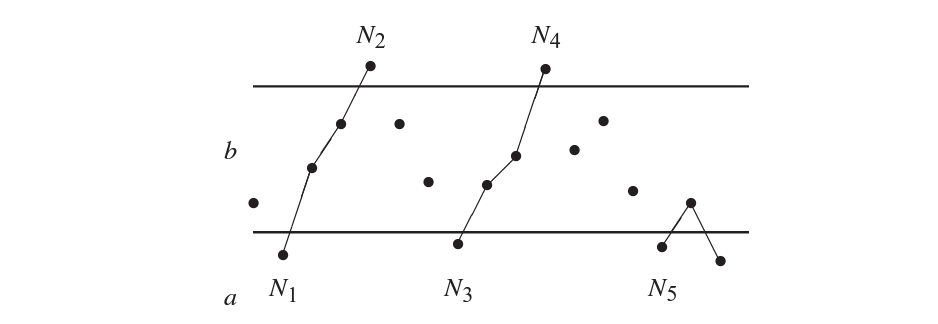
\includegraphics{StoppingTime.png}
		\item Every $N_j$ for $j\in \N$ is stopping time w.r.t $\{\F_n\}$. $N_1<N_2<N_3\cdots$ provided all $N_j$'s are finite. (It is possible that $N_j=\infty$ provided it has a form of $\inf(\phi)$)
		\item `Upcrossing' is a case where the submartingale $\{X_n\}$ crosses from below $a$ to above $b$.
		\item $\U_n:=\sup\{k\,:\, N_{2k}\leq n\}$ is the number of upcommings completed by time $n$
	\end{itemize}
	\item Upcrossing inequality
	\begin{itemize}
		\item Suppose $\{X_n\}$ is a submartingale w.r.t $\{\F_n\}$. If stopping time $N_j$ and the number of upcrossings $\U_n$ are defined as above then $$(b-a)E[\,\U_n]\leq E[(X_n-a)^+]-E[(X_0-a)^+]$$ 
	\end{itemize}
	\item Submartingale convergence theorem
	\begin{itemize}
		\item If $\{X_n\}$ is a submartingale w.r.t $\{\F_n\}$ with $\sup_n E(X_n^+)<\infty$ then $X_n\rightarrow X\;\, a.s.$ for some integrable random variable$X$
		\begin{itemize}
			\item[\trick] Trick : If $X_n\rightarrow X\;\, a.s.$ then $X_n^+\rightarrow X^+\;\,a.s.$ and $X_n^-\rightarrow X^-\;\,a.s.$
			\item[\trick] Lemma : If the number of upcrossings of $[a,b]$ by submartingale $\{X_n\}$ is finite for any $a,b\in \Q$, then $\lim_n X_n$ exists.\; i.e. $X_n$ converges to some r.v. almost surely.
		\end{itemize}
		\item[\sq] If $\{X_n\}$ is a nonnegative supermartingale w.r.t $\{\F_n\}$ then $X_n\rightarrow X\;\, a.s.$ for some integrable random variable $X$ s.t. $E(X)\leq E(X_0)$
	\end{itemize} 
	\item Example of martingale which converges almost surely but not in $L^1$
	\begin{itemize}
		\item $\{\xi_n\}_n\;i.i.d$ with $P(\xi_1=1)=P(\xi_1=-1)=1/2$. Let $S_0=1,\; S_n=S_{n-1}+\xi_n$ and $\F_0=\{\phi, \Omega\}, \; \F_n=\sigma(\xi_1, \cdots, \xi_n)$. Then $\{S_n\}$ is a martingale w.r.t $\{\F_n\}$ \\ Let $N=\inf\{n\in \N : S_n=0\}$. Then $N$ is a stopping time. \\ $X_n:=S_{N\wedge n}$ so that $X_n=S_n$ if $n<N$ and $X_n=0$ if $n\geq N$. $\{X_n\}$ is a nonnegative integer valued martingale w.r.t $\{\F_n\}$.\quad $X_n\rightarrow 0\;\, a.s.$ but $X_n \nrightarrow 0$ in $\LL^1$.
	\end{itemize}
	\item If $\{X_n\}_{n\in \N\cup\{0\}}$ is a negative submartingale w.r.t $\{\F_n\}_{n\in \N\cup\{0\}}$ then so is $\{X_n\}_{n\in \N\cup\{0,\infty\}}$ w.r.t $\{\F_n\}_{n\in \N\cup\{0,\infty\}}$ where $X_\infty=\lim_n X_n$ and $\F_\infty= \sigma\big(\bigcup_{n=0}^\infty \F_n \big)$



\end{itemize}

\end{document}